\section{Introduction} 
Nowadays, there exists huge amounts of spatiotemporal data in various fields of science.
% such as agriculture, transportation and social science.
Analysis of such data is interesting as it is grounded
on reality: each record represents a specific location and time. Moreover, understanding patterns and trends in this data provides analysis insights leading to improved user planning and decision making. Some instance applications of spatiotemporal data are smart city management, disaster management and autonomous transport \cite{RoddickEHPS04,Telang:2012}.

\begin{figure}[t]
  \centering
  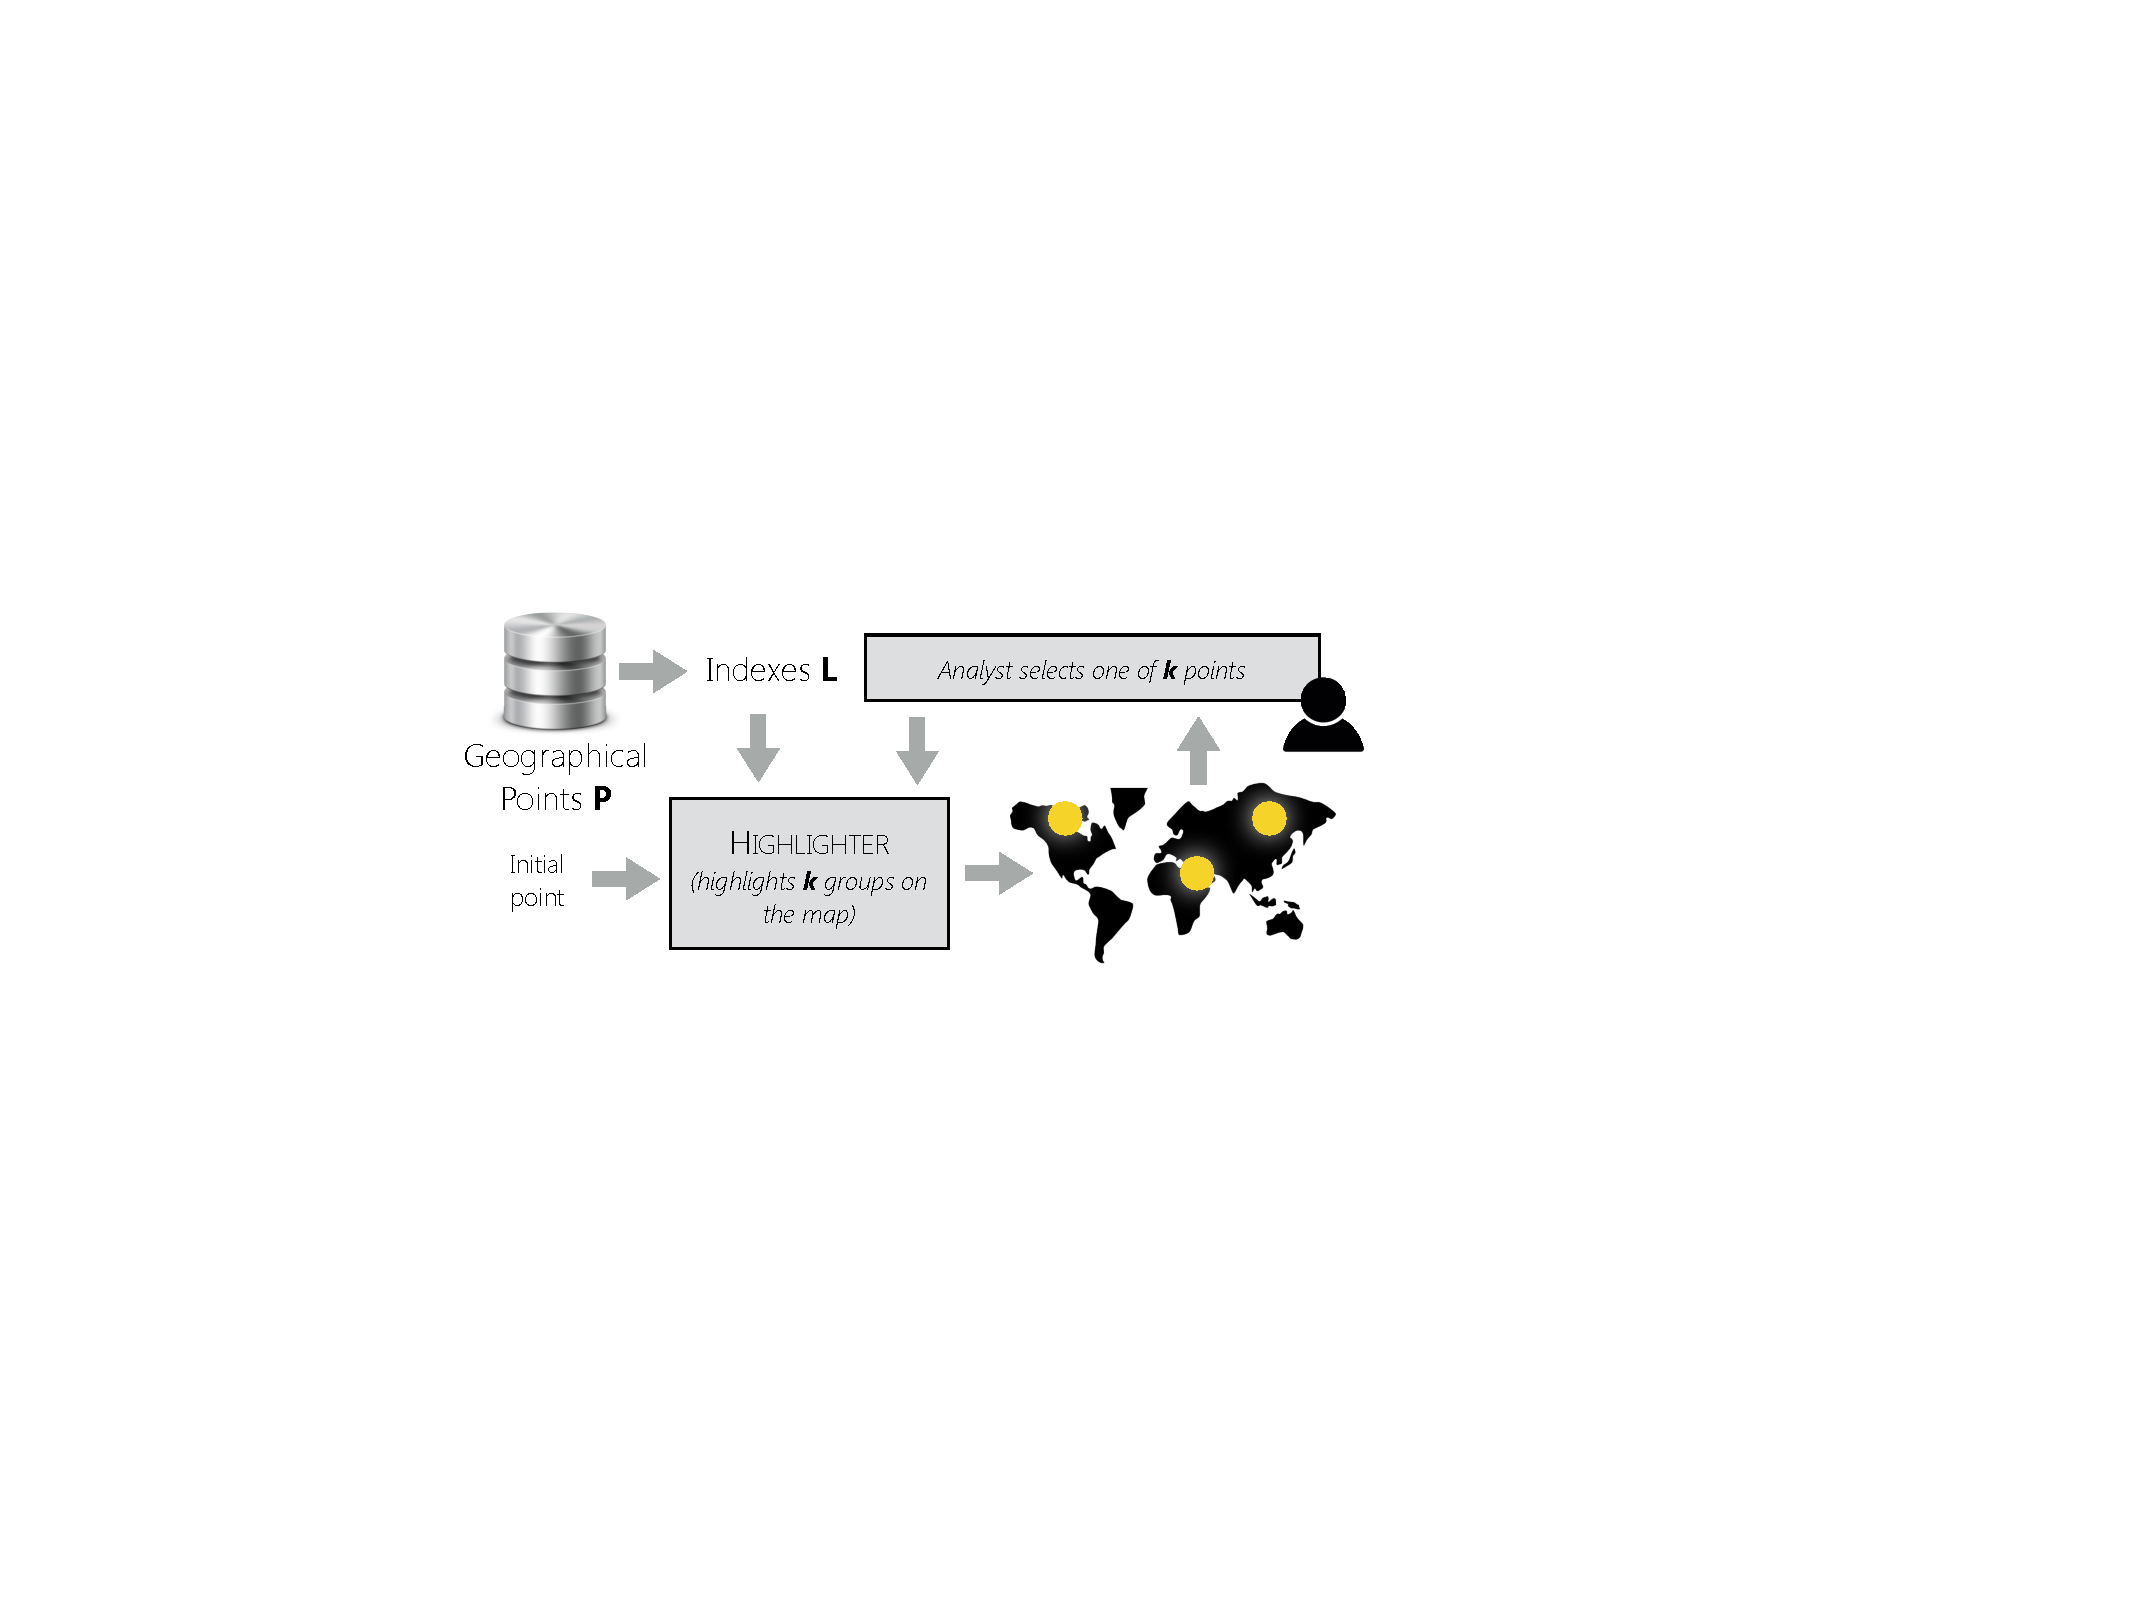
\includegraphics[width=\columnwidth]{figs/framework}
\caption{\framework\ Framework}
\label{fig:framework}
\end{figure}

Traditionally, an exploratory analysis scenario on spatiotemporal data is described as follows: the analyst visualizes the data using an off-the-shelf product (e.g., Tableau\footnote{\it http://www.tableau.com}, Exhibit\footnote{\it http://www.simile-widgets.org/exhibit/}, Spotfire\footnote{\it http://spotfire.tibco.com}, etc.). Then she looks at different parts of data for interesting patterns and trends. With the growing size of spatiotemporal datasets, this classical approach is not practical anymore: georgaphical points are scattered everywhere and the analyst cannot effectively observe patterns and trends.

To overcome this challenge, visualization environments offer a plethora of tools and operations to filter out data. In practice, this doubles the problem: the analyst is left alone in a huge space of data and operations. Considering the exploratory context as a non-idempotent process\footnote{\it We call an interactive step as ``idempotent'' if it always follows the exact same steps.}, the principled challenge for the analyst is {\em ``what to see next''} during the analysis process. A {\em guidance mechanism} is necessary for analysts to point out potential future directions of analysis.

Given a geographical point of interest, the question is then how to recommend other points to be considered in future analysis steps in form of guidance. In this paper, we focus on one specific guidance approach, i.e., highlighting $k$ best points given a point of interest. Those $k$ points should have high quality. Quality is formulated as optimization of two dimensions: {\em similarity} and {\em diversity}. Optimizing similarity ensures that recommended points are in-line with what the analyst has already liked. Optimizing diversity ensures that points are as different as possible from each other and unveils different aspects of analysis. Example \ref{ex:flight} illustrates a common case in practice.

\begin{example}
\label{ex:flight}
Tiffany is a data scientist and is tasked to design a {\em viral marketing} strategy for a Peking Duck product whose headquarters is in New York. She already knows that the product has success in the local area. So she analyzes Yelp spatiotemporal data\footnote{\it https://www.yelp.com/} (containing restaurant check-in records) to find out what other locations in the US exhibit similar eating profiles as New York. Hence, she asks for $k$ geographical points which have similar eating profile to New York and are the most diverse to cover the whole US. Given $k=3$, Tiffany receives points from San Fransisco, Washington DC and Marlton, NJ. She selects Marlton due its proximity to reduce transportation costs. Then she asks for other 3 best points for Marlton. This way she can make the city-to-city viral marketing strategy.
\end{example}

\noindent {\bf Challenges.} In this paper, we address the problem of guidance. Despite the great progress on spatiotemporal data analysis in recent years, we point out following challenges for guidance: $i.$ {\em Genericness.} Considering the heterogeneous nature of spatiotemporal datasets, it is challenging to come up with a generic guidance approach which is independent of data type and distribution. $ii.$ {\em Size}. The gigantic size of spatiotemporal datasets hinder discovery of possible interesting patterns and trends. The guidance approach should be able to provide a limited set of recommendations to overcome the problem of information overload. $iii.$ {\em Efficiency.} Guidance can be done efficiently in consecutive steps of analysis, so that the train of the analyst's thoughts won't break.

\vspace{5pt}
In this paper, we propose a generic interactive analysis approach for guiding analysts towards potential interesting points. The analyst can consider the guidance and choose a direction for the next iteration of analysis. 

% prune this
% \vspace{5pt}
% \noindent {\bf Outline.} in Section \ref{sec:data-model}, we present our data model. Then in Section \ref{sec:pb}, we formally define our problem. Section \ref{sec:algo} describes our solution for the guidance problem. We show a realistic application of our solution in Section \ref{sec:scenarios}. We present an extensive set of experiments in Section \ref{sec:exp}. A summary of related work is discussed in Section \ref{sec:rel}. Finally we conclude in Section \ref{sec:conc}.